\taskpic{ <<Тройник>> с двумя открытыми в атмосферу вертикальными
  трубками и одной закрытой (горизонтальная трубка) полностью заполнен
  водой. После того, как тройник стали двигать по горизонтали в
  плоскости рисунка влево с некоторым постоянным ускорением, из него
  вылилась 1/16 массы всей воды. Чему при этом стало равно давление в
  жидкости у закрытого конца, в точке $A$? Трубки имеют одинаковые
  внутренние сечения. Диаметр трубок мал по сравнению с
  $L$. Атмосферное давление равно $p_0$, плотность жидкости $\rho$. }
{
  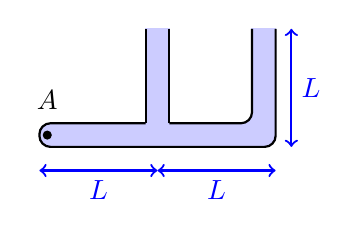
\begin{tikzpicture}
    \draw[blue!20,fill=blue!20] (1.85,0.2) rectangle (2.15,1.5);
    \draw[blue!20,fill=blue!20] (3.2,0.2) rectangle (3.5,1.5);
    \draw[blue!20,fill=blue!20, rounded corners] (1.85,0.3) -- (0.5,0.3) --
    (0.5,0) -- (3.5,0) -- (3.5,1.5) -- (3.2,1.5) -- (3.2,0.3) -- (2.15,0.3);
    \draw[thick, rounded corners] (1.85,0.3) -- (0.5,0.3) -- (0.5,0) --
    (3.5,0) -- (3.5,1.5);
    \draw[thick, rounded corners] (3.2,1.5) -- (3.2,0.3) -- (2.15,0.3);
    \draw[thick] (2.15,0.3) -- (2.15,1.5) (1.85,0.3) -- (1.85,1.5);
    \draw[blue,thick,<->] (2,-0.3) -- (0.5,-0.3)
    node[midway,below,blue] {$L$};
    \draw[blue,thick,<->] (2,-0.3) -- (3.5,-0.3)
    node[midway,below,blue] {$L$};
    \draw[blue,thick,<->] (3.7,0) -- (3.7,1.5) node[right,midway,blue]
    {$L$};
    \draw[fill=black] (0.6,0.15) circle (0.05) node[above=0.2cm] {$A$};
  \end{tikzpicture}
}
% Квант, 2006, №1
